\section{Failure Mechanism}
\label{sec:failure}

Placeholder, budget 1.25 pages. The docking envelope sweep (Fig.~\ref{fig:pdock}), the failed 8~s trial (Fig.~\ref{fig:trajectory}), and the offline decomposition of the recorded trials (Fig.~\ref{fig:mech}): the world-frame measurement is within 1~cm of truth, the velocity state is accurate while markers are visible, the feedforward over-drives the plant with the identified gain and lag, and the blackout dead-reckoning that produces the apparent phantom velocity. The loop argument uses the plant gain and lag identified in the step tests.

\begin{figure}[t]
  \centerline{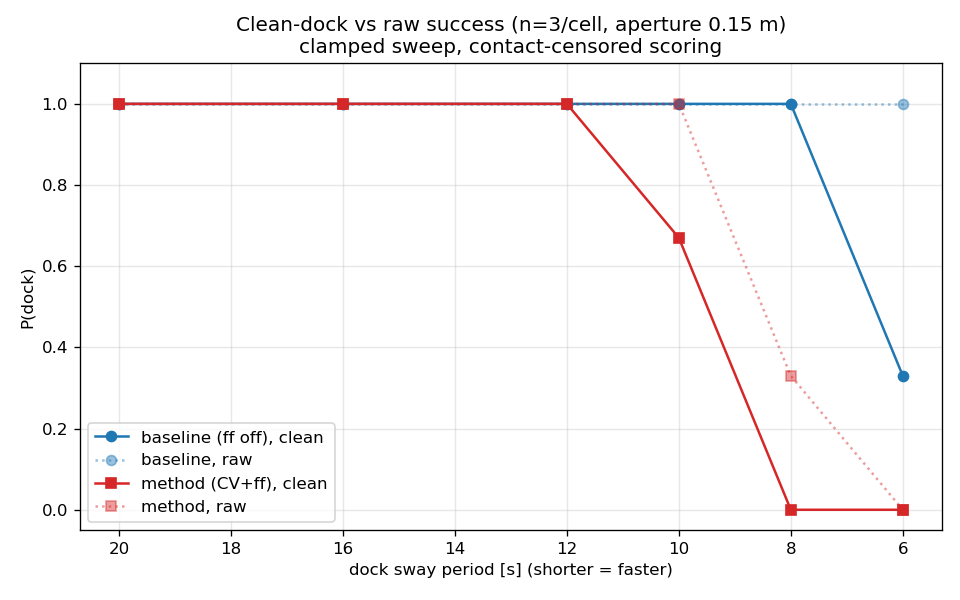
\includegraphics[width=0.7\columnwidth]{figures/clean_pdock.png}}
  \caption{Docking success versus sway period, reactive baseline versus constant-velocity filter with feedforward; raw (dotted) and contact-censored (solid) scoring.}
  \label{fig:pdock}
\end{figure}

\begin{figure}[t]
  \centerline{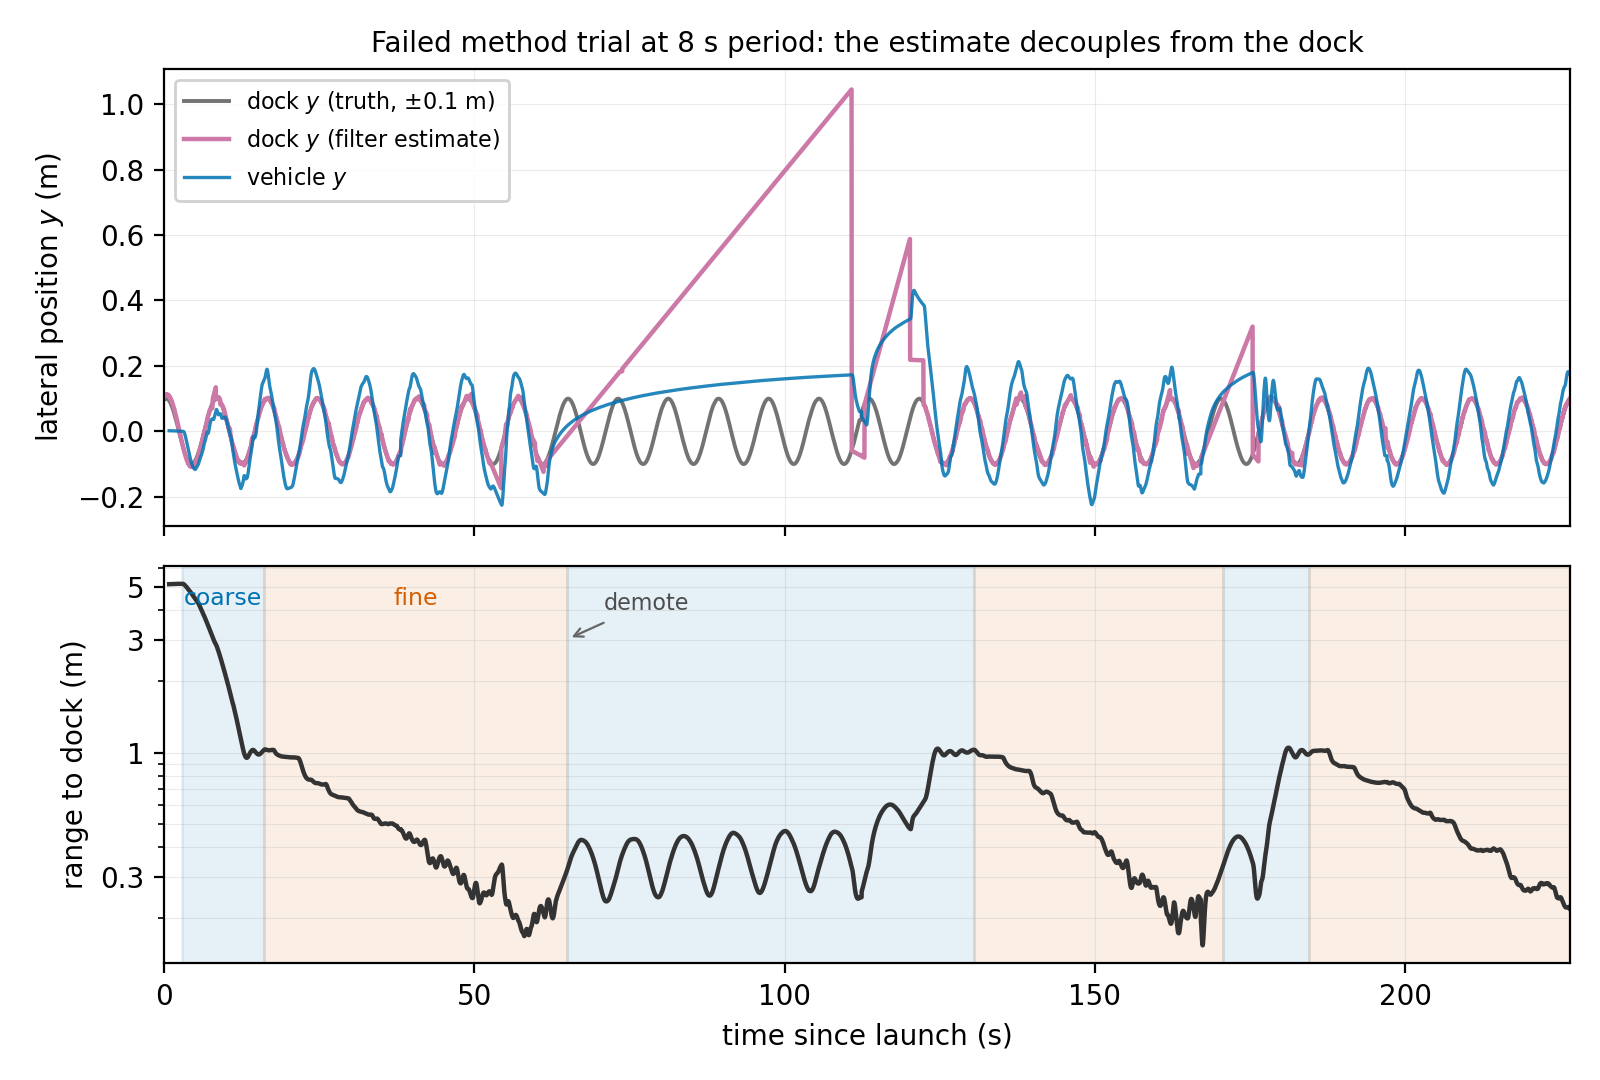
\includegraphics[width=0.75\columnwidth]{figures/rov_trajectory_failure.png}}
  \caption{Failed feedforward trial at 8~s. Top: lateral position of the true dock, the estimate and the vehicle. Bottom: range to the dock with phases shaded.}
  \label{fig:trajectory}
\end{figure}

\begin{figure}[t]
  \centerline{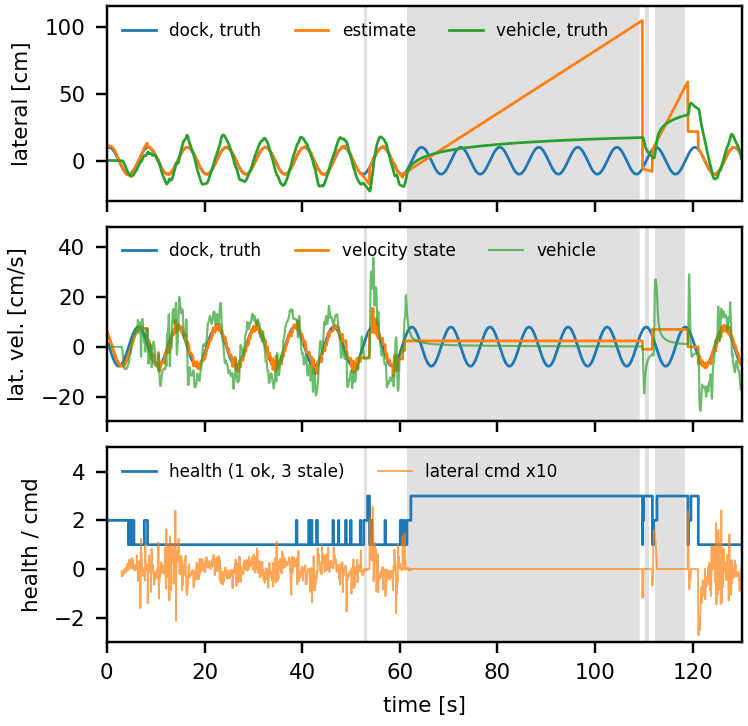
\includegraphics[width=0.95\columnwidth]{figures/mechanism_p8.png}}
  \caption{Decomposition of the failed 8~s trial. Top: the estimate sits on the dock while the vehicle over-swings, then dead-reckons when markers are lost (shaded). Middle: the velocity state tracks the true dock velocity; the vehicle's is twice it. Bottom: filter health and lateral command; the command is zero throughout the blackout.}
  \label{fig:mech}
\end{figure}
